% Capstan RL Field Guide: how the v4 quadruped learns, read from the code (rl2/).
% Build: latexmk -pdf rl-field-guide.tex   (pdflatex; TeX Live 2024+)
\documentclass[10pt,letterpaper]{article}
\usepackage[T1]{fontenc}
\usepackage[utf8]{inputenc}
\usepackage{newtxtext,newtxmath}
\usepackage[scaled=0.95]{zi4}
\usepackage[margin=0.72in,top=0.7in,bottom=0.8in]{geometry}
\usepackage{microtype}
\DisableLigatures[-]{encoding=T1,family=tt*}
\usepackage[dvipsnames]{xcolor}
\usepackage{tikz}
\usetikzlibrary{arrows.meta,positioning,calc,fit,backgrounds}
\usepackage{booktabs,tabularx,array,multicol}
\usepackage{listings}
\usepackage{enumitem}
\usepackage{titlesec}
\usepackage[most]{tcolorbox}
\usepackage{amsmath}
\usepackage[colorlinks=true,linkcolor=Accent,urlcolor=Accent,citecolor=Accent]{hyperref}

\definecolor{Accent}{HTML}{1C5CAB}
\definecolor{Scan}{HTML}{12A596}
\definecolor{Teach}{HTML}{2A78D6}
\definecolor{Stud}{HTML}{EB6834}
\definecolor{Blind}{HTML}{1BAF7A}
\definecolor{Ink2}{HTML}{4C5660}
\definecolor{Code}{HTML}{F3F5F7}
\definecolor{Rule}{HTML}{D3D9DE}

\setlist{itemsep=1pt,topsep=2pt,parsep=0pt,leftmargin=1.3em}
\setlength{\parindent}{0pt}
\setlength{\parskip}{4pt}
\titleformat{\section}{\large\bfseries\sffamily\color{Accent}}{\thesection}{0.6em}{}
\titleformat{\subsection}{\normalsize\bfseries\sffamily}{\thesubsection}{0.5em}{}
\titlespacing*{\section}{0pt}{12pt}{4pt}
\titlespacing*{\subsection}{0pt}{8pt}{2pt}

\lstset{basicstyle=\ttfamily\footnotesize, backgroundcolor=\color{Code}, frame=none, xleftmargin=4pt, xrightmargin=4pt,
  aboveskip=4pt, belowskip=4pt, columns=fullflexible, keepspaces=true, showstringspaces=false, language=Python,
  keywordstyle=\color{Accent}\bfseries, commentstyle=\color{Ink2}\itshape, stringstyle=\color{BrickRed}, upquote=true,
  literate={→}{{$\rightarrow$}}1 {−}{{$-$}}1 {²}{{$^2$}}1}

\newcommand{\repo}{https://github.com/soujanya957/capstan-drive-leg/blob/231ca53/CapstanPedal/fullbuild_v4}
\newcommand{\gh}[2]{\href{\repo/#1\##2}{\texttt{\detokenize{#1}}\,\textsuperscript{\tiny #2}}}
\newcommand{\ghf}[1]{\href{\repo/#1}{\texttt{\detokenize{#1}}}}
\newcommand{\cc}[1]{\texttt{\detokenize{#1}}}
\newcommand{\key}[1]{\textbf{#1}}
\newtcolorbox{note}[1][]{colback=Accent!5,colframe=Accent!60,boxrule=0.5pt,arc=2pt,left=5pt,right=5pt,top=3pt,bottom=3pt,fontupper=\small,#1}
\newtcolorbox{warn}{colback=BrickRed!5,colframe=BrickRed!60,boxrule=0.5pt,arc=2pt,left=5pt,right=5pt,top=3pt,bottom=3pt,fontupper=\small}

\begin{document}

\begin{center}
{\sffamily\bfseries\LARGE Capstan RL Field Guide}\\[3pt]
{\sffamily How the v4 quadruped learns to move, read from the code}\\[2pt]
{\small\color{Ink2} \texttt{CapstanPedal/fullbuild\_v4/rl2} \;·\; 26 October 2026 \;·\; code links point at commit \href{https://github.com/soujanya957/capstan-drive-leg/tree/231ca53}{\texttt{231ca53}}; the teacher–student code (§\ref{sec:ts}) is newer}
\end{center}

\begin{note}
\textbf{The whole thing in one paragraph.} A URDF made from the CAD becomes a MuJoCo simulation. 8{,}192 copies of the robot
run at once on the GPU. Every 20\,ms each robot's \emph{policy} (a neural network) reads 153 noisy sensor numbers and outputs
12 joint targets, plus random noise so it tries something slightly different each time. Every step is scored by a weighted sum
of reward terms. A second network, the \emph{critic}, predicts how much reward is coming. After 24 steps of all 8{,}192 robots,
PPO makes the actions that did \emph{better than the critic expected} more likely and the rest less likely. Repeat 1{,}500
times (about 15–30 minutes on the RTX 4090) and the noise becomes a walk. Only the policy runs on the robot.
\end{note}

\tableofcontents

% =====================================================================================================================
\section{The map}

\begin{center}
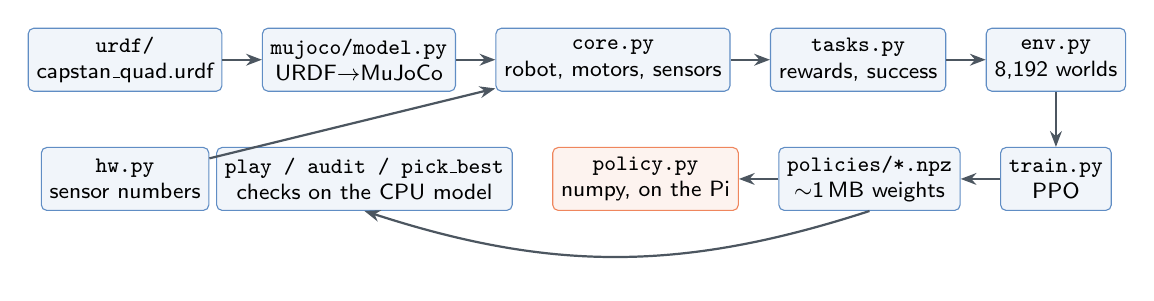
\begin{tikzpicture}[node distance=4mm and 5mm, every node/.style={font=\footnotesize\sffamily},
  box/.style={draw=Accent!70, fill=Accent!6, rounded corners=2pt, minimum height=8mm, align=center, inner sep=3pt},
  run/.style={draw=Stud!80, fill=Stud!8, rounded corners=2pt, minimum height=8mm, align=center, inner sep=3pt},
  ar/.style={-{Stealth[length=2mm]}, thick, color=Ink2}]
\node[box] (u) {\texttt{urdf/}\\capstan\_quad.urdf};
\node[box, right=of u] (m) {\texttt{mujoco/model.py}\\URDF$\to$MuJoCo};
\node[box, right=of m] (c) {\texttt{core.py}\\robot, motors, sensors};
\node[box, right=of c] (t) {\texttt{tasks.py}\\rewards, success};
\node[box, right=of t] (e) {\texttt{env.py}\\8{,}192 worlds};
\node[box, below=7mm of e] (tr) {\texttt{train.py}\\PPO};
\node[box, left=of tr] (np) {\texttt{policies/*.npz}\\$\sim$1\,MB weights};
\node[run, left=of np] (p) {\texttt{policy.py}\\numpy, on the Pi};
\node[box, left=of p] (chk) {\texttt{play / audit / pick\_best}\\checks on the CPU model};
\node[box, below=7mm of u] (hw) {\texttt{hw.py}\\sensor numbers};
\draw[ar] (u)--(m); \draw[ar] (m)--(c); \draw[ar] (c)--(t); \draw[ar] (t)--(e); \draw[ar] (e)--(tr); \draw[ar] (tr)--(np);
\draw[ar] (np)--(p); \draw[ar] (np.south) to[bend left=18] (chk.south); \draw[ar] (hw)--(c);
\end{tikzpicture}
\end{center}

Everything for the learned controller lives in \texttt{rl2/}. It borrows the robot from two folders next to it:
\texttt{urdf/} (the description generated from CAD) and \texttt{mujoco/} (which turns the URDF into a simulation and also
holds the hand-written controller \texttt{gait.py}). \texttt{rl/} is the first version (walking only, ideal sensors); read \texttt{rl2}.

\begin{small}
\begin{tabularx}{\linewidth}{@{}>{\raggedright\ttfamily}p{3.6cm}X@{}}
\toprule
\normalfont\textbf{File} & \textbf{Its job} \\ \midrule
hw.py & The sensors as numbers: 50\,Hz policy, 4–20\,ms delay, gyro noise, encoder resolution, optical-flow dropouts, battery sag. Replace the assumed values with measurements. \\
core.py & Builds the model twice (light ``physics'' for the GPU, ``full'' with every mesh for checking); PD loop and motor model; \cc{sense()}, which turns true simulator state into what the sensors would report; terrain height. \\
tasks.py & The five tasks (walk, terrain, rear, handstand, balance): what an episode is, the scenario bank, every reward term, success and fall. \\
env.py & Steps a task: \cc{GpuEnv} runs thousands of worlds on the GPU, \cc{CpuEnv} one world in the full model. \\
train.py & PPO: actor and critic, rollout, update, logging, held-out evaluation, snapshots. \cc{--teacher=1}: a teacher (§\ref{sec:ts}). \\
distill.py & Teacher $\to$ blind student by imitation (DAgger). No reward. \\
policy.py & The trained actor in numpy. This is what would run on the Raspberry Pi. \\
play.py, audit.py, pick\_best.py & Held-out success on the full model, stress tests, choosing the best snapshot. \\
terms.py, progress.py, showreel.py, compare\_film.py & Looking at runs: which reward terms dominated, films of snapshots, the all-skills film, teacher/student/blind side by side. \\
run\_queue.sh, experiments/ & Train a batch on cake; every batch we ran is a list file. \\
check\_robot.py & Does a build's robot fit rl2? (§\ref{sec:build}) \\
wandb\_sync.py & Streams the CSV logs to Weights \& Biases; training itself needs no account. \\ \bottomrule
\end{tabularx}
\end{small}

% =====================================================================================================================
\section{From a URDF to 8,192 robots on a GPU}

\begin{enumerate}[leftmargin=1.4em]
\item \key{Read the URDF as XML.} \gh{mujoco/model.py}{L33-L46} parses \texttt{capstan\_quad.urdf} and pulls out the
\texttt{<mimic>} tags: the motor rotors spin at $-9\times$ their output, and MuJoCo cannot read mimic, so they come back later as
joint equalities.
\begin{lstlisting}
root = ET.parse(urdf).getroot()
for j in root.findall("joint"):
    m = j.find("mimic")
    ...
spec = mujoco.MjSpec.from_string(ET.tostring(root, encoding="unicode"))
\end{lstlisting}
\item \key{Add what a URDF cannot say} (\gh{mujoco/model.py}{L48-L125}): a free joint so the torso can fly (URDF roots are fixed),
a floor and lights, 12 actuators (motor C on ab/ad, B on the hip, A on the crank), the four-bar loop closed with a
\emph{connect} equality, reflected rotor inertia (\emph{armature}) on the driven joints, and foot sites.
\item \key{Make the learning version.} \cc{core.build_spec("physics")} (\gh{rl2/core.py}{L60-L98}) deletes every visual mesh and
the rotor joints: the GPU only needs collision shapes, and the rotor inertia is already in the armature. The ``full'' version
keeps everything and adds the flow and range sensor boards. Tasks add \emph{extras}: 64 mocap boxes for the terrain course, or a ball and board.
\item \key{Find things by name.} \cc{Layout} (\gh{rl2/core.py}{L115-L146}) records where the 12 driven joints, four feet and the
torso are in the compiled model, and computes the standing pose from the leg IK in \texttt{gait.py}. This is why a new build works as long as the names stay.
\item \key{Copy it onto the GPU} (\gh{rl2/env.py}{L26-L42}). \cc{GpuEnv} compiles the model and hands it to MuJoCo Warp through MJX;
one \texttt{Data} per robot, all stepped together with \cc{jax.vmap}. Friction, mass and the terrain differ per robot, so they are passed per world.
\end{enumerate}

% =====================================================================================================================
\section{One step of one robot}

A \emph{step} is one decision, 50 times per simulated second. Between decisions physics runs 10 times (500\,Hz) with the joint
PD loop holding the targets.

\subsection{What the policy sees: 3 frames of 51 numbers}
Every number passes through \cc{sense()} (\gh{rl2/core.py}{L216-L241}), so it is noisy, biased, late, quantised or missing, as on the robot.

\begin{small}
\begin{tabularx}{\linewidth}{@{}lrX@{}}
\toprule
\textbf{Group} & \textbf{n} & \textbf{Source on the robot, and the sim's errors} \\ \midrule
Rotation rate (gyro) $\times0.25$ & 3 & pi3hat IMU; 0.02\,rad/s noise, $\pm$0.02\,rad/s bias per episode \\
Gravity direction & 3 & pi3hat attitude filter; $\pm1.5^\circ$ tilt error per episode, $0.4^\circ$ noise \\
Ground speed (fwd, side) $\times2$ & 2 & PMW3901 optical flow $\times$ range: one step old, $\pm$8\,\% scale, dropouts held, 15\,\% of episodes dead \\
Flow valid & 1 & the flow sensor's quality flag \\
Height $(h-h_0)\times5$ & 1 & VL53L1X time-of-flight range; 5\,mm + 1\,\% noise \\
Command & 3 & joystick: forward, sideways (m/s), turn (rad/s); scaled $\times2, \times2, \times0.25$ \\
Joint angles $-$ standing pose & 12 & moteus encoders: 14-bit through 9:1, $\pm$0.01\,rad calibration offset \\
Joint speeds $\times0.05$ & 12 & moteus velocity estimate, 0.05\,rad/s noise \\
Last action & 12 & the policy's own previous output \\
Trot clock & 2 & $\sin, \cos$ of a 0.3\,s cycle (walking tasks; zeros otherwise) \\ \bottomrule
\end{tabularx}
\end{small}

Three frames are stacked (153 numbers), so the policy can see short trends. Each input is then normalised by a running mean
and variance and clipped to $\pm10$.

\subsection{Act, with noise}
The actor is an MLP, $153\to512\to256\to128\to12$ with ELU activations. It outputs a mean $\mu(o)$; during training a Gaussian
sample is taken with a learned, state-independent standard deviation $\sigma=e^{\texttt{log\_std}}$ (initially $e^{-1}\approx0.37$):
\[
a \sim \mathcal{N}\big(\mu_\theta(o),\ \mathrm{diag}\,\sigma^2\big),\qquad
\log \pi_\theta(a\mid o)=\sum_{j=1}^{12}\Big[-\tfrac12\Big(\tfrac{a_j-\mu_j}{\sigma_j}\Big)^2-\log\sigma_j-\tfrac12\log2\pi\Big].
\]
\begin{lstlisting}
mu = actor_mean(p, nm, obs)
std = jp.exp(p["log_std"])
a = mu + std * jax.random.normal(k_a, mu.shape)     # each robot gets its own noise: exploration
\end{lstlisting}
On the robot (and in every evaluation) the noise is off: the action is $\mu(o)$.

\subsection{Action $\to$ joint targets $\to$ torque}
Each action moves a joint target from the standing pose: 0.2\,rad per unit on ab/ad, 0.6 on hip and crank, clamped to the
firmware limits (\gh{rl2/core.py}{L187-L193}). For 10 sub-steps the PD loop and motor model (\gh{rl2/env.py}{L51-L70}) compute
\[
\tau = k_p(q^\ast-q) - k_d\,\dot q,\qquad
|\tau| \le \tau_{\max}\, s\;\mathrm{clip}\Big(2\big(1-\tfrac{|\dot q|}{\omega_0 b}\big),0,1\Big),
\]
with $k_p=80/60/60$, $k_d=1.5/2/2$ per joint, $s$ the motor strength (0.75–1.05 per episode), $b$ the battery sag (0.83–1.0), and
the crank output A limited further by how hard the coupler can push. Full torque up to half the no-load speed, falling to zero at it.
The new targets only apply after the episode's control delay (4–20\,ms); before that the old ones hold.
\begin{lstlisting}
tgt = jp.where(i < delay, aux["prev_target"], target)
tau = C.torque(jp, pos, vel, tgt, aux["kp"], aux["kd"], aux["strength"], aux["w0"], L.isA)
d = mjx.step(mx, d.replace(ctrl=d.ctrl.at[L.act].set(tau)))
\end{lstlisting}

\subsection{Score it}
The task's \cc{end()} reads the \emph{true} state (the simulator knows everything; the policy does not), computes every
reward term, decides fallen / success / time-out, and senses the next observation (\gh{rl2/tasks.py}{L166-L194} for walk,
\gh{rl2/tasks.py}{L118-L133} for the shared \cc{finish()}).

% =====================================================================================================================
\section{Did that noisy try get reward? The critic, the advantage, PPO}

Reward arrives \emph{every step}; there is no separate check at the end. \cc{finish()} multiplies each raw term by its weight
and adds them up, then scales by 0.1:
\[ r_t = 0.1\sum_k w_k\, x_{k,t}. \]
Success and falls are terms in this sum ($+10$, $-10$), not a separate signal: PPO never looks at ``success'' on its own.

\subsection{Return and value}
What we want to maximise is the \emph{discounted return}, the reward from here on with later rewards counted less:
\[
G_t=\sum_{l\ge0}\gamma^l r_{t+l},\qquad \gamma=0.99 \;\;(\text{a reward 100 steps = 2\,s ahead counts }0.99^{100}\approx0.37).
\]
The \emph{critic} $V_\phi(s)$ learns to predict $G_t$. It may read things the robot cannot (the 22 \emph{privileged} numbers:
true velocity, true height, foot contacts, friction, added mass, motor strength, gains, delay, flow scale error, and per task
6 more; terrain now reads a 30-point height scan and foot clearances instead). The critic only exists in training, so this is allowed.

\subsection{Advantage: better or worse than expected?}
A balanced, standing robot always collects decent reward; that says nothing about whether its last action was good. So PPO asks
whether the outcome beat the critic's prediction:
\[ A_t \approx G_t - V(s_t). \]

\begin{small}
\begin{tabularx}{\linewidth}{@{}lXrrrX@{}}
\toprule
Robot & Its noise pushed it\ldots & Expected & Got & Advantage & PPO will\ldots \\ \midrule
\#17 & front-left foot down a bit earlier & 0.80 & 1.00 & $+0.20$ & make that action more likely \\
\#4{,}203 & hip harder, body pitched & 0.80 & 0.50 & $-0.30$ & make it less likely \\
\#6{,}050 & about the mean & 0.80 & 0.81 & $+0.01$ & barely change \\ \bottomrule
\end{tabularx}
\end{small}

\subsection{GAE: estimating the advantage from 24 steps}
After a 24-step rollout we do not know $G_t$ (episodes are 400 steps). \emph{Generalised advantage estimation} mixes
real rewards with the critic's guess of the rest, walking backwards (\gh{rl2/train.py}{L304-L311}):
\[
\delta_t = r_t + \gamma\,(1-d_t)\,V(s_{t+1}) - V(s_t),\qquad
\hat A_t = \delta_t + \gamma\lambda\,(1-d_t)\,\hat A_{t+1},\qquad \lambda=0.95,
\]
where $d_t=1$ if the episode ended at $t$ (no future after a fall). The critic's training target is $\hat R_t=\hat A_t+V(s_t)$.
One subtlety: a \emph{time-out} is not a real ending (the robot would have kept going), so on a time-out the code adds
$\gamma V(s_{t+1})$ to the reward: it bootstraps from the last state instead of treating the future as zero.
\begin{lstlisting}
def gae(nxt, t):
    adv_n, v_n = nxt
    nd = 1.0 - t["done"]                              # no future after a fall
    delta = t["r"] + o["gamma"] * v_n * nd - t["v"]   # reward + expected next - expected now
    adv = delta + o["gamma"] * o["lam"] * nd * adv_n
    return (adv, t["v"]), adv
\end{lstlisting}

\subsection{The PPO update}
For each stored action, the \emph{ratio} $\rho_t(\theta)=\pi_\theta(a_t\mid o_t)/\pi_{\text{old}}(a_t\mid o_t)$ says how much more
likely the new network makes it than the one that chose it. With advantages normalised per minibatch
($\hat A\leftarrow(\hat A-\bar A)/\mathrm{sd}(\hat A)$), PPO minimises (\gh{rl2/train.py}{L283-L294})
\[
L(\theta,\phi)=-\,\mathbb{E}_t\Big[\min\big(\rho_t\hat A_t,\ \mathrm{clip}(\rho_t,1-\epsilon,1+\epsilon)\,\hat A_t\big)\Big]
+ c_v\,\mathbb{E}_t\big[(V_\phi(s_t)-\hat R_t)^2\big] - c_e\,\mathcal{H}[\pi_\theta],
\]
with $\epsilon=0.2$, $c_v=1$, $c_e=0.004$. The clip stops one batch from moving the policy more than $\pm20\,\%$ on any action;
the entropy bonus $\mathcal{H}=\sum_j(\log\sigma_j+\tfrac12\log2\pi e)$ keeps some exploration. Each iteration makes 5 passes
over the batch in 4 minibatches of 49{,}152, with Adam and gradient-norm clipping at 1.

\textbf{Adaptive learning rate} (\gh{rl2/train.py}{L365-L368}): the approximate KL divergence
$\mathbb{E}[(\rho-1)-\log\rho]$ measures how far one update moved the policy. Above $2\times0.01$ the learning rate is divided
by 1.5; below $0.01/2$ it is multiplied by 1.5 (bounds $10^{-5}$–$10^{-2}$).

\begin{note}
\textbf{One try teaches almost nothing.} The policy moves because 196{,}608 noisy actions per update average out toward the
better ones. Any single robot's experience is mostly noise.
\end{note}

% =====================================================================================================================
\section{What happens next: four loops}

\begin{small}
\begin{tabularx}{\linewidth}{@{}llX@{}}
\toprule
\textbf{Word} & \textbf{How long} & \textbf{What it is here} \\ \midrule
Step & 20\,ms & One action, 10 physics steps, one reward. \\
Episode & $\le$400 steps & One try at one scenario: walk 8\,s, poses 6\,s. Ends early on a fall, or (terrain) on reaching the goal. \\
Iteration & 24 steps & Every robot takes 24 steps ($8{,}192\times24=196{,}608$ samples), then one PPO update. \\
Run & $\sim$1{,}500–2{,}000 iterations & One training job: 300–400\,M steps, 15–30 minutes on the 4090 at 200–235\,k steps/s. \\ \bottomrule
\end{tabularx}
\end{small}

The weights are fixed during the 24-step rollout and change only at the update. Episodes do \emph{not} restart at an update: a
robot halfway through a walk keeps walking with the slightly better policy. When a robot's episode ends it is reset in the same
step into a new scenario. All robots run in lock-step on the GPU, so the reset is a \emph{masked swap}: where \texttt{done} is
true take the fresh state, else keep the old (\cc{GpuEnv.respawn}).
\begin{lstlisting}
new_cfg = jax.random.randint(k_c, (n,), 0, n_cfg)          # uniform; or SGS / curriculum
d2, aux2, mp, obs_n, priv_n = env.respawn(bank, d2, aux2, mp, obs2, priv2, done, new_cfg, k_r)
# inside: sel = lambda new, old: jp.where(done[:, None...], new, old)
\end{lstlisting}

A \emph{scenario} is one row of the \emph{bank}: everything random about an episode, fixed in advance. Commands, floor friction
(0.4–1.25), added mass ($-0.5$ to $+2$\,kg), motor strength, gain errors, battery sag, a shove (time and velocity), and for
terrain the course itself. 1{,}040 scenarios for training; 4{,}160 different ones (another seed) for the held-out test.

\subsection{Choosing the next scenario}
\begin{itemize}
\item \key{Uniform}: any scenario, equally likely. What every deployable policy used.
\item \key{SGS} (success-guided sampling, Zhang et al.\ 2026): each scenario keeps its last 100 outcomes; with $p_i$ their mean,
\[ w_i=\max\big((p_i+\varepsilon)^{kt}(1-p_i+\varepsilon)^{k(1-t)},\ \varepsilon\big),\quad P(i)\propto \exp\big(\log(w_i+\varepsilon)/T\big),\quad t=0.66,\ k=5,\ T=2, \]
which peaks at scenarios succeeded about two times in three: hard but possible.
\item \key{Level curriculum} (Rudin et al.\ 2021): each robot keeps a level per terrain type, up one on success, down one on failure.
\end{itemize}
\textbf{What we found}: over 14 runs SGS never beat uniform and lost 15–20 points on terrain (a scenario that fails early is
sampled less, so it is never learned: the bank \emph{freezes}). The curriculum gave $+3$ points, within seed noise; robots settled
at level $\sim$1, because up-on-success/down-on-failure settles where success is 50\,\%.

% =====================================================================================================================
\section{Logs and saving}

\begin{small}
\begin{tabularx}{\linewidth}{@{}l>{\ttfamily}p{4.6cm}X@{}}
\toprule
\textbf{When} & \normalfont\textbf{File (on cake)} & \textbf{What is in it} \\ \midrule
Start & logs/<name>\_opts.json & Every option and the reward weights used: a run can always be reproduced. \\
Every iteration & logs/<name>.csv & Steps, speed, learning rate, mean reward, success and fall rate of finished episodes, KL, critic loss, noise size, every reward term as \texttt{r.<term>}. \\
Every 10 it. & logs/<name>.out & A printed line with the four biggest reward terms. \\
Every 50 it. & logs/<name>\_eval.jsonl & Held-out test: 4{,}160 unseen scenarios, mean action, success per terrain and level. \\
Every 50 it. & policies/snaps/<name>/<M>.npz & An actor snapshot (teacher runs also keep a \texttt{.pkl}). \\
Every 50 it., end & policies/<name>.npz, .pkl & \texttt{.npz}: actor + input normalisation, $\sim$1\,MB, deployable. \texttt{.pkl}: everything, to resume. \\
After the run & logs/<name>.post, .audit, .pick & \texttt{run\_queue.sh} films it, evaluates it on the full CPU model, stress-tests it, picks the best snapshot as \texttt{<name>\_best.npz}. \\ \bottomrule
\end{tabularx}
\end{small}

Only the deployable \texttt{\_best.npz} files live in git; logs, checkpoints and films stay on cake.
\texttt{wandb\_sync.py --follow} streams the CSVs to Weights \& Biases while a run trains.

% =====================================================================================================================
\section{Base RL: the reward you actually care about}

The plainest reward is the goal itself: $+10$ for success, $-10$ for a fall, nothing otherwise. That is \emph{sparse} (base)
reward, and it is in every task as the \texttt{success} and \texttt{fall} terms. On its own it almost never works for a legged
robot: a random policy falls within a second, every time, never stumbles into an 8\,s walk that tracks the command, so success is
never seen and the only lesson is ``falling is bad''. The policy learns to crouch and sit still.

% =====================================================================================================================
\section{Reward shaping: terms that point the way}

Shaping adds \emph{dense} terms that give partial credit every step, so a slightly better policy gets slightly more reward long
before it ever succeeds. The whole walk reward (\gh{rl2/tasks.py}{L141-L142} weights, \gh{rl2/tasks.py}{L170-L181} raw values,
\gh{rl2/tasks.py}{L111-L116} shared terms):

\begin{small}
\begin{tabularx}{\linewidth}{@{}>{\ttfamily}lXrX@{}}
\toprule
\normalfont\textbf{Term} & \textbf{Raw value each step} & \textbf{Weight} & \textbf{Why} \\ \midrule
track\_lin & $\exp(-\lVert v_{xy}-c_{xy}\rVert^2/0.25)$ & $+1.5$ & The goal as partial credit \\
track\_yaw & $\exp(-(\omega_z-c_\omega)^2/0.25)$ & $+0.75$ & Turning on command \\
gait & share of feet whose contact matches the trot clock & $+0.5$ & Asks for a trot (§\ref{sec:gaits}) \\
air & at touch-down: air time $-$ 0.15\,s & $+1.0$ & Real steps, not shuffling \\
bounce & $v_z^2$ & $-2.0$ & Smooth body \\
angvel & $\omega_x^2+\omega_y^2$ & $-0.05$ & No rocking \\
tilt & $g_x^2+g_y^2$ (gravity off vertical) & $-5.0$ & Body level \\
height & $(z-z_{\text{stand}})^2$ & $-20$ & No crouch-walking \\
torque & $\sum\tau^2$ & $-2{\times}10^{-4}$ & Energy, motor heat \\
action\_rate & $\sum(a_t-a_{t-1})^2$ & $-0.01$ & No jitter: gears would suffer \\
slip & $\sum$ speed$^2$ of feet in contact & $-0.2$ & Planted feet \\
idle\_pose & distance from standing pose, when the command is zero & $-0.2$ & Stand still properly \\
fall & 1 on the step it falls & $-10$ & Base reward \\
success & 1 at the end of a successful episode & $+10$ & Base reward \\ \bottomrule
\end{tabularx}
\end{small}

\subsection{Why a bell curve}
Tracking terms use $\exp(-e^2/\sigma)$ rather than $-e^2$: full credit at the target, smoothly less further away, never a cliff,
and bounded, so one term cannot drown the rest. With $\sigma=0.25$:
error 0 $\to$ 1.00; 0.25\,m/s $\to$ 0.78; 0.5\,m/s $\to$ 0.37; 1\,m/s $\to$ 0.02. At 0.25\,m/s off, track\_lin pays
$0.78\times1.5\times0.1=0.117$ per step, about 47 over an 8\,s episode, against the $\pm1$ of success/fall after scaling: the
dense terms carry most of the signal.

\subsection{Shaping in the other tasks}
\textbf{Rear, handstand}: \texttt{pose} pays for the nose pointing up (down) as a bell curve around the target angle;
\texttt{feet} pays for the right pair being off the ground; \texttt{roll}, \texttt{drift} are penalties (\gh{rl2/tasks.py}{L343-L344}).
\textbf{Balance}: \texttt{alive} pays 1 per step not fallen, \texttt{board\_level} penalises a tilted board, \texttt{feet\_on} pays
for feet on the board (\gh{rl2/tasks.py}{L417-L418}). \textbf{Terrain}: the walk terms with gentler tilt and height penalties,
so stairs and slopes are not punished (\gh{rl2/tasks.py}{L279-L280}).

\begin{warn}
\textbf{The policy optimises what you wrote, not what you meant.} The first handstand held the body at 45–50°, right at the 50°
success bar, because the pose bell curve paid nearly as much there as at 64°. ``Successful'' 14\,\% of the time. That is a shaping bug.
\end{warn}

% =====================================================================================================================
\section{Reward tuning: picking the numbers}

Shaping picks the terms; tuning picks their weights (and widths such as the 0.25). The loop:
\begin{enumerate}
\item Train with the current weights.
\item Watch the film and read the term report (\cc{python terms.py walk walk_try}): which term dominates, which never moved.
\item Find the term that pays for the wrong thing or does not punish it enough. Change one or two weights.
\item Retrain without editing code: \cc{python train.py --task=walk --w=slip=-0.5,air=2.0 --name=walk_try}. An unknown term name is
an error (\gh{rl2/tasks.py}{L50-L55}), so typos cannot silently do nothing.
\end{enumerate}

\begin{small}
\begin{tabularx}{\linewidth}{@{}XXX@{}}
\toprule
\textbf{What we saw} & \textbf{What changed} & \textbf{Result} \\ \midrule
Handstand hovering at the 50° bar & pose target $0.90\to0.87$ ($\approx$\,60°), width $0.15\to0.05$, new \texttt{margin} term (+1.0) rising smoothly from 50° to 58° & best snapshot 35\,\% $\to$ 82\,\% \\
Handstand resting on the body's front edge & a body corner touching the ground counts as a fall & no more leaning \\
Torque constraint 85\,\% (\texttt{--cat=0.25}) & episodes cut when a motor passed 85\,\% & 0\,\%: the working handstand needs more than 85\,\% on 41\,\% of steps. Too strict a number kills the skill \\ \bottomrule
\end{tabularx}
\end{small}

\textbf{Tuning is not the only lever.} Walk fell 3 times in 4 when the flow sensor died. That was fixed by training with it dead in
15\,\% of episodes (\texttt{hw.FLOW\_DEAD}): falls $75\,\%\to0\,\%$. That is \emph{domain randomisation}: changing what the robot
practises rather than what it is paid for.

% =====================================================================================================================
\section{An RL controller vs the model-based one}

Both send joint targets to the same PD loop and motor model; they differ in how they choose them.

\begin{multicols}{2}
\textbf{\texttt{mujoco/gait.py}: written by a person.}
\begin{itemize}
\item Picks a gait from a table: which feet are down when.
\item Plans each foot: stance feet slide back at the commanded speed; swing feet land where the Raibert rule says (half a stride
ahead, corrected for speed error), lifted on an arc.
\item Leg inverse kinematics turns foot positions into joint angles.
\item Feed-forward force $J^\top F$ so each stance leg carries its share of the weight, plus roll and pitch correction.
\item Uses the true body state from the simulator.
\item Predictable and explainable; does only what its author thought of. No handstand, no board on a ball; an unplanned shove or step can tip it.
\end{itemize}
\columnbreak
\textbf{\texttt{rl2}: found by trial and error.}
\begin{itemize}
\item One network: 153 sensor numbers in, 12 joint targets out, 50 times a second.
\item No foot planning, no IK, no gait table: the stepping pattern is whatever the reward favoured.
\item Sees only the noisy, late readings the real robot will have.
\item Trained on thousands of variations (friction, mass, weak motors, shoves, delay), so it copes with them.
\item Does skills that are hard to write by hand (handstand, balance board, blind stairs). Cannot explain itself, can find loopholes in the reward, and is only as good as the simulation is honest.
\end{itemize}
\end{multicols}

% =====================================================================================================================
\section{Continuous commands}

Both controllers take the same three joystick numbers: forward and sideways speed (m/s) and turn rate (rad/s). They are continuous:
any mix, any value in range. A diagonal walk is two at once, e.g.\ forward 0.4, sideways 0.3.

\textbf{In \texttt{gait.py}} the command goes straight into the foot plan: stance feet slide backwards along the command vector
(diagonally, for a diagonal) and the Raibert rule places swing feet ahead along it. The diagonal works because the geometry says so.

\textbf{In the RL policy} the command is 3 of the 51 numbers in each frame. The policy has no idea what they mean; it learns that
\texttt{track\_lin} pays when its body speed equals them. It can walk diagonally because it was trained on diagonals: forward
$-0.5\ldots1.2$, sideways $-0.4\ldots0.4$, turn $-1.2\ldots1.2$, 30\,\% along one axis only, 12\,\% standing still, switching to new
values 4\,s into each episode (\gh{rl2/tasks.py}{L143-L158}). Consequence: the policy is only good inside the ranges it saw. Ask for
2\,m/s and it will do \emph{something}, but nobody rewarded it. Ranges are a training choice, not physics.

In \textbf{terrain} a simulated operator gives the commands: speed ramps to the target, sideways and turn commands steer back to the
course's centre line (\gh{rl2/tasks.py}{L328}). In \texttt{teleop.py} the keyboard sets them.

% =====================================================================================================================
\section{How does it know trot vs walk vs crawl?}\label{sec:gaits}

It does not, unless the reward says so. A gait is a timing pattern: which feet are down at each moment of the stride. Given only
``track the speed, do not fall'', RL finds whatever pattern pays most: maybe a trot, maybe a bound, a pronk, or a shuffle the
simulator allows and a real robot should not do. The walk task asks for a trot two ways:
\begin{enumerate}
\item \key{A clock in the input}: the last 2 numbers of each frame are $\sin,\cos$ of a 0.3\,s cycle, so the policy knows where in
the stride it is.
\item \key{A reward for following it}: \texttt{gait} pays the share of feet whose contact matches the clock. Pod $i$ has phase offset
$o_i$; it should be down while $(\phi+o_i)\bmod 1 < d$, with duty $d=0.5$.
\end{enumerate}
\begin{lstlisting}
OFF = np.array([0.5, 0.0, 0.0, 0.5])     # per pod: LF, LR, RF, RR -> diagonal pairs: a trot
want = (phase + C.OFF) % 1.0 < 0.5       # True = this foot should be on the ground
gait = jp.mean(contact == want)
\end{lstlisting}
(The robot walks toward $-X$, so the ``F'' pods are its hind legs.) Other gaits are other offsets and duties; these are the ones
\texttt{gait.py} uses (bars: foot on the ground, two strides):

\begin{center}
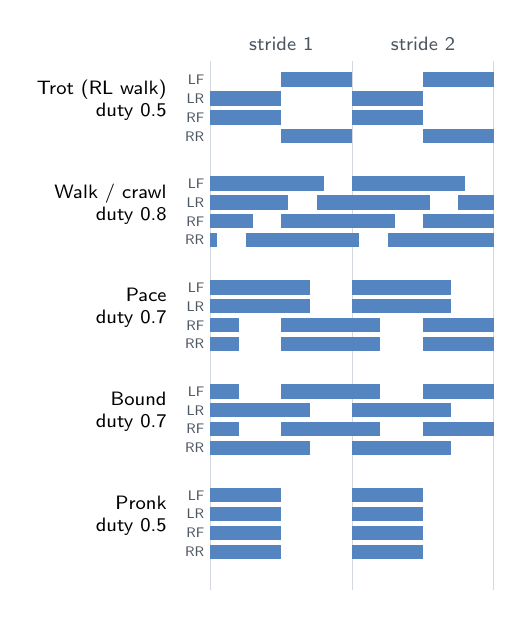
\begin{tikzpicture}[x=3.6cm, y=0.24cm, every node/.style={font=\scriptsize\sffamily}]
\def\gaitrow#1#2#3#4#5#6#7{% name, ystart, duty, LF, LR, RF, RR
  \node[anchor=north east, align=right] at (-0.12, #2) {#1};
  \foreach \p/\o [count=\k] in {LF/#4, LR/#5, RF/#6, RR/#7} {
    \pgfmathsetmacro{\yy}{#2-\k}
    \node[anchor=east, color=Ink2, inner sep=1pt] at (-0.01, \yy+0.5) {\tiny\p};
    \foreach \c in {-1,0,1,2} {
      \pgfmathsetmacro{\s}{\c - \o}
      \pgfmathsetmacro{\e}{\s + #3}
      \pgfmathsetmacro{\ss}{max(0,\s)} \pgfmathsetmacro{\ee}{min(2,\e)}
      \pgfmathparse{\ee > \ss ? 1 : 0}
      \ifnum\pgfmathresult=1 \fill[Accent!75] (\ss/2, \yy+0.12) rectangle (\ee/2, \yy+0.88); \fi
    }
  }
}
\draw[Rule] (0,0.5) -- (0,-27.5); \draw[Rule] (0.5,0.5) -- (0.5,-27.5); \draw[Rule] (1,0.5) -- (1,-27.5);
\gaitrow{Trot (RL walk)\\duty 0.5}{0}{0.5}{0.5}{0}{0}{0.5}
\gaitrow{Walk / crawl\\duty 0.8}{-5.5}{0.8}{0}{0.25}{0.5}{0.75}
\gaitrow{Pace\\duty 0.7}{-11}{0.7}{0}{0}{0.5}{0.5}
\gaitrow{Bound\\duty 0.7}{-16.5}{0.7}{0.5}{0}{0.5}{0}
\gaitrow{Pronk\\duty 0.5}{-22}{0.5}{0}{0}{0}{0}
\node[color=Ink2] at (0.25, 1.4) {stride 1}; \node[color=Ink2] at (0.75, 1.4) {stride 2};
\end{tikzpicture}
\end{center}

Three ways to get gaits from RL, from most control to least:
\begin{enumerate}
\item \key{Fix one gait} with a clock and a gait reward, as here. For a crawl: offsets $(0, 0.25, 0.5, 0.75)$ and duty 0.75 so three
feet are always down (today the 0.5 duty is written into the \texttt{want} line, so it would become a parameter).
\item \key{Make the gait a command}: put offsets and duty in the observation, draw a different gait per episode; one policy learns
them all and the operator picks at run time (``Walk These Ways'', Margolis and Agrawal 2022).
\item \key{Let it emerge}: drop the gait terms, keep an energy penalty. Fu et al.\ (2021) found energy alone gives a walk at low
speed, a trot at medium and a gallop-like gait at high, as animals do. Less control over what you get.
\end{enumerate}

% =====================================================================================================================
\section{Privileged learning: a teacher that sees, a student that feels}\label{sec:ts}

\textbf{The idea} (Lee et al.\ 2020, ``Learning quadrupedal locomotion over challenging terrain''; Kumar et al.\ 2021, RMA).
Learning to walk blind over terrain is hard partly because the policy has to work out the ground from its legs \emph{and} learn to
act on it, at once, from a noisy reward. Split the two:

\begin{center}
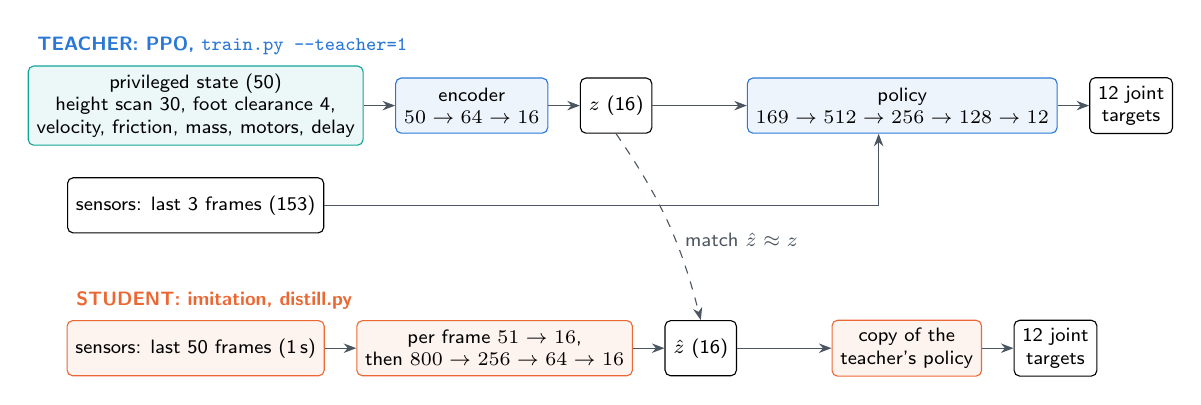
\begin{tikzpicture}[node distance=3mm and 4mm, every node/.style={font=\scriptsize\sffamily},
  b/.style={draw, rounded corners=2pt, align=center, inner sep=3pt, minimum height=7mm},
  ar/.style={-{Stealth[length=1.6mm]}, color=Ink2}]
\node[b, draw=Scan, fill=Scan!8] (pv) {privileged state (50)\\height scan 30, foot clearance 4,\\velocity, friction, mass, motors, delay};
\node[b, draw=Teach, fill=Teach!8, right=of pv] (enc) {encoder\\$50\to64\to16$};
\node[b, right=of enc] (z) {$z$ (16)};
\node[b, below=4mm of pv] (ob) {sensors: last 3 frames (153)};
\node[b, draw=Teach, fill=Teach!8, right=12mm of z] (act) {policy\\$169\to512\to256\to128\to12$};
\node[b, right=of act] (a) {12 joint\\targets};
\draw[ar] (pv)--(enc); \draw[ar] (enc)--(z); \draw[ar] (z)--(act); \draw[ar] (ob.east) -| ($(act.south)+(-3mm,0)$); \draw[ar] (act)--(a);
\node[b, draw=Stud, fill=Stud!8, below=11mm of ob] (h) {sensors: last 50 frames (1\,s)};
\node[b, draw=Stud, fill=Stud!8, right=of h] (henc) {per frame $51\to16$,\\then $800\to256\to64\to16$};
\node[b, right=of henc] (zh) {$\hat z$ (16)};
\node[b, draw=Stud, fill=Stud!8, right=12mm of zh] (act2) {copy of the\\teacher's policy};
\node[b, right=of act2] (a2) {12 joint\\targets};
\draw[ar] (h)--(henc); \draw[ar] (henc)--(zh); \draw[ar] (zh)--(act2); \draw[ar] (act2)--(a2);
\node[anchor=west, color=Teach, font=\scriptsize\bfseries\sffamily] at ($(pv.north west)+(0,2.5mm)$) {TEACHER: PPO, \texttt{train.py -{}-teacher=1}};
\node[anchor=west, color=Stud, font=\scriptsize\bfseries\sffamily] at ($(h.north west)+(0,2.5mm)$) {STUDENT: imitation, distill.py};
\draw[dashed, color=Ink2, ar] (z.south) to[bend left=10] node[right, pos=0.6] {match $\hat z \approx z$} (zh.north);
\end{tikzpicture}
\end{center}

\textbf{Teacher.} Ordinary PPO, but its policy also reads the privileged state through a small encoder to a 16-number latent $z$.
For terrain that state is a height scan of the course (10 points from 0.3\,m behind to 1.05\,m ahead $\times$ 3 across, relative to
the body's height), each foot's height above the ground under it, and the hidden physics (true velocity, friction, added mass, motor
strength, gains, delay). The robot has no sensor for any of it, so the teacher is not deployable: \texttt{policy.py} refuses it.

\textbf{Student.} Blind. It reads the last 50 frames (1\,s) of the robot's real sensors. A shared per-frame layer ($51\to16$)
compresses each frame; an MLP over the 50 compressed frames estimates $\hat z$; the policy is initialised as a \emph{copy} of the
teacher's and reads $[$last 3 frames$, \hat z]$. Trained by imitation, with no reward at all:
\[
\mathcal{L}=\mathbb{E}_{s\sim d^{\pi_\beta}}\Big[\lVert \pi_S(h_s)-\mu_T(o_s,p_s)\rVert^2+\lVert \hat z(h_s)-z(p_s)\rVert^2\Big],
\qquad \pi_\beta=\begin{cases}\mu_T & \text{with prob. }\beta\\ \pi_S & \text{otherwise}\end{cases},
\]
where $h$ is the 1\,s history, $p$ the privileged state, and $\beta$ falls from 1 to 0 over the first 20\,\% of training.
This is \textbf{DAgger} (Ross et al.\ 2011): the states come from the \emph{student's own} driving, so it learns what to do after
its own mistakes, which plain copying of teacher trajectories never shows it.

\textbf{What happened} (Experiment 5, \texttt{experiments/queue5.list}, 26 Oct 2026; all held-out):

\begin{small}
\begin{tabularx}{\linewidth}{@{}Xrrrrr@{}}
\toprule
& Peak, GPU (4{,}160) & Best snap., CPU (200) & Last snap., CPU (200) & Stress audit (240) & Gaps (GPU) \\ \midrule
\textcolor{Teach}{\textbf{Teacher}} (sees the scan) & \textbf{80.9\,\%} & not deployable & -- & -- & \textbf{52\,\%} \\
\textcolor{Stud}{\textbf{Student}} (blind, distilled) & 78.3\,\% & 77.0\,\% & \textbf{74.5\,\%} & \textbf{76\,\%} & 12\,\% \\
\textcolor{Blind}{\textbf{Blind PPO}} (control) & 70.7\,\% & 77.0\,\% & 55.5\,\% & 59\,\% & 11\,\% \\ \bottomrule
\end{tabularx}
\end{small}

\begin{itemize}
\item \key{Seeing is worth about 10 points, nearly all on gaps and mixed courses.} A blind robot cannot know a gap is there until a
foot finds nothing; no imitation can fix that. In the films the teacher lengthens its stride before the gap; student and blind both
stop at the edge.
\item \key{The student keeps what can be felt}: stairs up 86\,\% vs 74\,\% blind; rough, slope, obstacles slightly better.
\item \key{Best against best, blind success did not move} (77.0\,\% both, $\pm$3 points at 200 episodes).
\item \key{Distillation is stable where PPO is not.} The teacher slumped 81 $\to$ 45\,\%, the blind run 71 $\to$ 55\,\%; the student
stayed in 63–78\,\% throughout. Supervised learning has a fixed target, which points the late-slump problem at the RL loop itself.
\item \key{Next}: give the robot part of the scan. A forward-facing 8$\times$8-zone range sensor (VL53L5CX) would let a student see gaps coming.
\end{itemize}

% =====================================================================================================================
\section{Is it good? How a policy is judged}

\begin{itemize}
\item \key{Held-out, noise off.} Training success is measured with exploration noise on scenarios being trained on. The number that
counts is success on scenarios never trained on, with the mean action.
\item \key{The full model.} Training runs in the light GPU model; every reported score is re-measured in the full CPU model (every mesh,
rotors on their joints), which the policy never saw.
\item \key{Pick the snapshot, not the last iterate.} Held-out success swings $\pm15$ points between evaluations 40\,M steps apart and often
sags late. \texttt{pick\_best.py} plays the top GPU snapshots on a separate CPU \emph{selection} bank, keeps the winner, and only then
\texttt{play.py eval} gives the test number. This was the biggest single gain: terrain 50.5 $\to$ 73.5\,\% (3 seeds), handstand 10 $\to$ 82\,\%.
\item \key{Stress audit} (\texttt{audit.py}): worst-case sensors, weak motors, slippery floor, dead flow sensor.
\item \key{Seeds.} One run is one sample; differences under $\sim$5 points between single runs are noise.
\end{itemize}

% =====================================================================================================================
\section{A new build version}\label{sec:build}

\texttt{rl2} never names v4: it reads the robot from the folder it sits in (\cc{core.BUILD}, or \cc{CAPSTAN_BUILD=<path>}).
\begin{enumerate}
\item Build v5 as usual (CAD $\to$ meshes $\to$ \texttt{urdf/build\_urdf.py}), keeping the names: \texttt{torso}, \texttt{foot\_LF}\ldots\texttt{foot\_RR}, rotor joints \texttt{*\_rotor*}.
\item Copy the code: \cc{rsync -a --exclude policies --exclude logs fullbuild_v4/rl2/ fullbuild_v5/rl2/}.
\item Check it: \cc{JAX_PLATFORMS=cpu python check_robot.py --policy=walk2_best}. Names, both models, standing on PD alone, sensors in
range, and whether an old policy still walks. If that fails, retrain.
\item If the robot changed a lot, revisit the v4-tuned numbers: PD gains and action range in \texttt{core.py}, sensor values in
\texttt{hw.py}, fall heights and pose targets in \texttt{tasks.py}.
\item Train on cake: \cc{sh run_queue.sh experiments/<batch>.list}. Films come out as \texttt{video/v5\_rl2\_*.mp4}.
\end{enumerate}

% =====================================================================================================================
\section{Words}

\begin{small}
\begin{tabularx}{\linewidth}{@{}>{\bfseries}p{3.4cm}X@{}}
\toprule
Policy / actor & The network that picks actions; the only part that runs on the robot. \\
Critic / value & Predicts future reward. Training only, so it may read privileged state. \\
Return & Sum of future rewards, each step ahead counted $0.99\times$ less. \\
Advantage & Return actually got minus what the critic expected. Positive: do that more. \\
GAE & Advantage estimate mixing real rewards with the critic's guess; $\lambda$ trades bias for variance. \\
Entropy, \texttt{log\_std} & How much noise the policy adds to explore. Learned; a bonus keeps it from collapsing early. \\
KL & How far one update moved the policy; used to adapt the learning rate. \\
Sparse / dense reward & Paid only at the end (success, fall) vs every step (tracking, posture). \\
Shaping / tuning & Choosing reward terms / choosing their weights. \\
Domain randomisation & Training on many versions of the world so the policy works on the real one. \\
Scenario bank & Fixed list of episode settings; training draws from one, testing uses another. \\
Privileged information & What the simulator knows and the robot cannot sense (terrain ahead, friction). \\
Teacher–student, DAgger & Train with privileged info, then imitate it from real sensors, on the student's own states. \\
Held-out evaluation & Testing on scenarios never trained on, without noise. The only fair score. \\
Sim-to-real gap & Everything the simulation gets wrong about the robot; \texttt{hw.py} exists to shrink it. \\ \bottomrule
\end{tabularx}
\end{small}

\vspace{4pt}
{\small\color{Ink2} Results, films and the whole run history: \texttt{rl2/sgs-lessons.md}; the results pages on claude.ai; the
\texttt{capstan-rl2} project on Weights \& Biases.}

\end{document}
